\documentclass{article}
\usepackage{amsmath}
\usepackage{enumerate}
\usepackage{listings}
\usepackage{moreverb}
\usepackage[margin=1in]{geometry}
\usepackage{graphicx}
\usepackage{dsfont}
\title{STA 360: Lab 5}
\author{Michael Lin}

\begin{document}
\maketitle

\begin{enumerate}
\item Given $\beta\sim$Uniform(0,1), $N \sim$Poisson$(\lambda)$, and $y\sim$Binomial$(N,\beta)$, they have the following prior distributions:
\begin{align*}
&p(\beta) = \mathds{1}(0\leq \beta \leq 1) \\
&p(N) = \frac{\lambda^N}{N!}e^{-\lambda} \\
&p(y|N,\beta) = \binom{N}{y} \beta^y(1-\beta)^{N-y}
\end{align*}

Therefore, the joint posterior distribution is:
\begin{align*}
p(N,\beta|y) &= p(y|N,\beta)p(\beta)p(N) \\
&= \binom{N}{y}\beta^y(1-\beta)^{N-y}\cdot \mathds{1}(0\leq \beta \leq 1)\cdot \frac{\lambda^N}{N!}e^{-\lambda} \\
&= \frac{N!}{y!(N-y)!}\beta^y(1-\beta)^{N-y}\frac{\lambda^N}{N!}e^{-\lambda} \\
&= \frac{\lambda^N e^{-\lambda}}{y!(N-y)!}\beta^y(1-\beta)^{N-y} \\
&=\Big(\frac{\beta}{1-\beta}\Big)^y\frac{(1-\beta)^N \lambda^N e^{-\lambda}}{y!(N-y)!}
\end{align*}

\item Marginal distribution of $N$. First, we find the marginal distribution of $N-y$:
$$ p(N-y | y,\beta) \propto \frac{[(1-\beta)\lambda]^{(N-y)+y}}{(N-y)!} \propto \text{Poisson}((1-\beta)\lambda) $$
Thus, the marginal distribution of $N$ is:
$$ p(N | y,\beta) = y + \text{Poisson}((1-\beta)\lambda) $$

Marginal distribution of $\beta$.
$$ p(\beta | y,N) \propto \Big(\frac{\beta}{1-\beta}\Big)^y(1-\beta)^N = \beta^y(1-\beta)^{N-y} \propto \text{Beta}(y+1, N-y+1) $$
Thus, the marginal distribution of $\beta$ is:
$$ p(\beta | y,N)=\text{Beta}(y+1, N-y+1)$$

\item See R code

\item Graphs for Gibbs sampling are shown below. \\
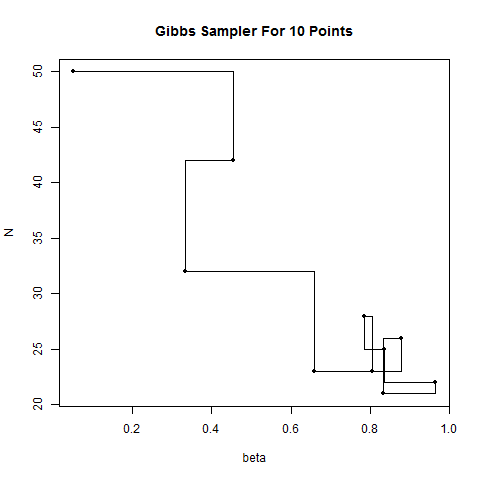
\includegraphics[scale = 0.45]{gibb10.png}
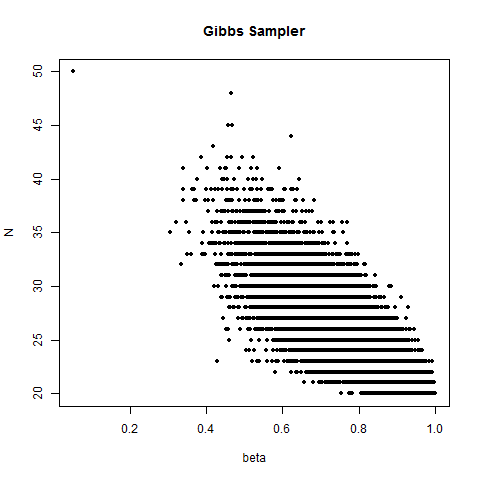
\includegraphics[scale=0.45]{gibb.png}

\item Using the \texttt{quantile} function, we found the 90 \% posterior credible interval to be:
$$(0.55,0.97)$$

\item The probability that exactly 20 people were polled is 0.073.


\end{enumerate}
\pagebreak
\listinginput[1]{1}{lab5.r}
\end{document}